\chapter{Implementation - Computer Vision}

This chapter will cover the implementation methods on computer vision side of this project using either ASUS Xtion or ZED Mini. By adjusting some settings which will be discussed in this chapter, the algorithm works for both cameras. The entire code for this part can be seen in !!!!!!!!!!

\section{Camera Setup}
The dependency package allow specific camera to communicate with ROS is shown in Table \ref{camerapackage}, which contains corresponding launch files. Entering the launch command in the terminal can start the package driver. After that, a list of camera topics including RGB, depth, and point-clouds etc can be subscribed for further processing. 

\begin{table}[H]
\centering
\resizebox{\columnwidth}{!}{
\begin{tabular}{||c||c|c||}
\hline
Camera & Dependency package & Launch command \\ \hline \hline
ASUS Xtion & $openni2$ & $roslaunch$ $openni2\_launch$ $openni2.launch$ \\ \hline
ZED Mini & $zed-ros-wrapper$ & $roslaunch$ $zed\_wrapper$ $zedm.launch$ \\ \hline
\end{tabular}
}
\caption{The dependency packages and launch commands for Cameras}
\label{camerapackage}
\end{table}

In ROS, video streams are represented by these sequences of images. If user would like to use ROS images in conjunction with OpenCV, $CvBridge$ package provides the converting interface, which is used in this project as well.

\begin{figure}[H]
\centering
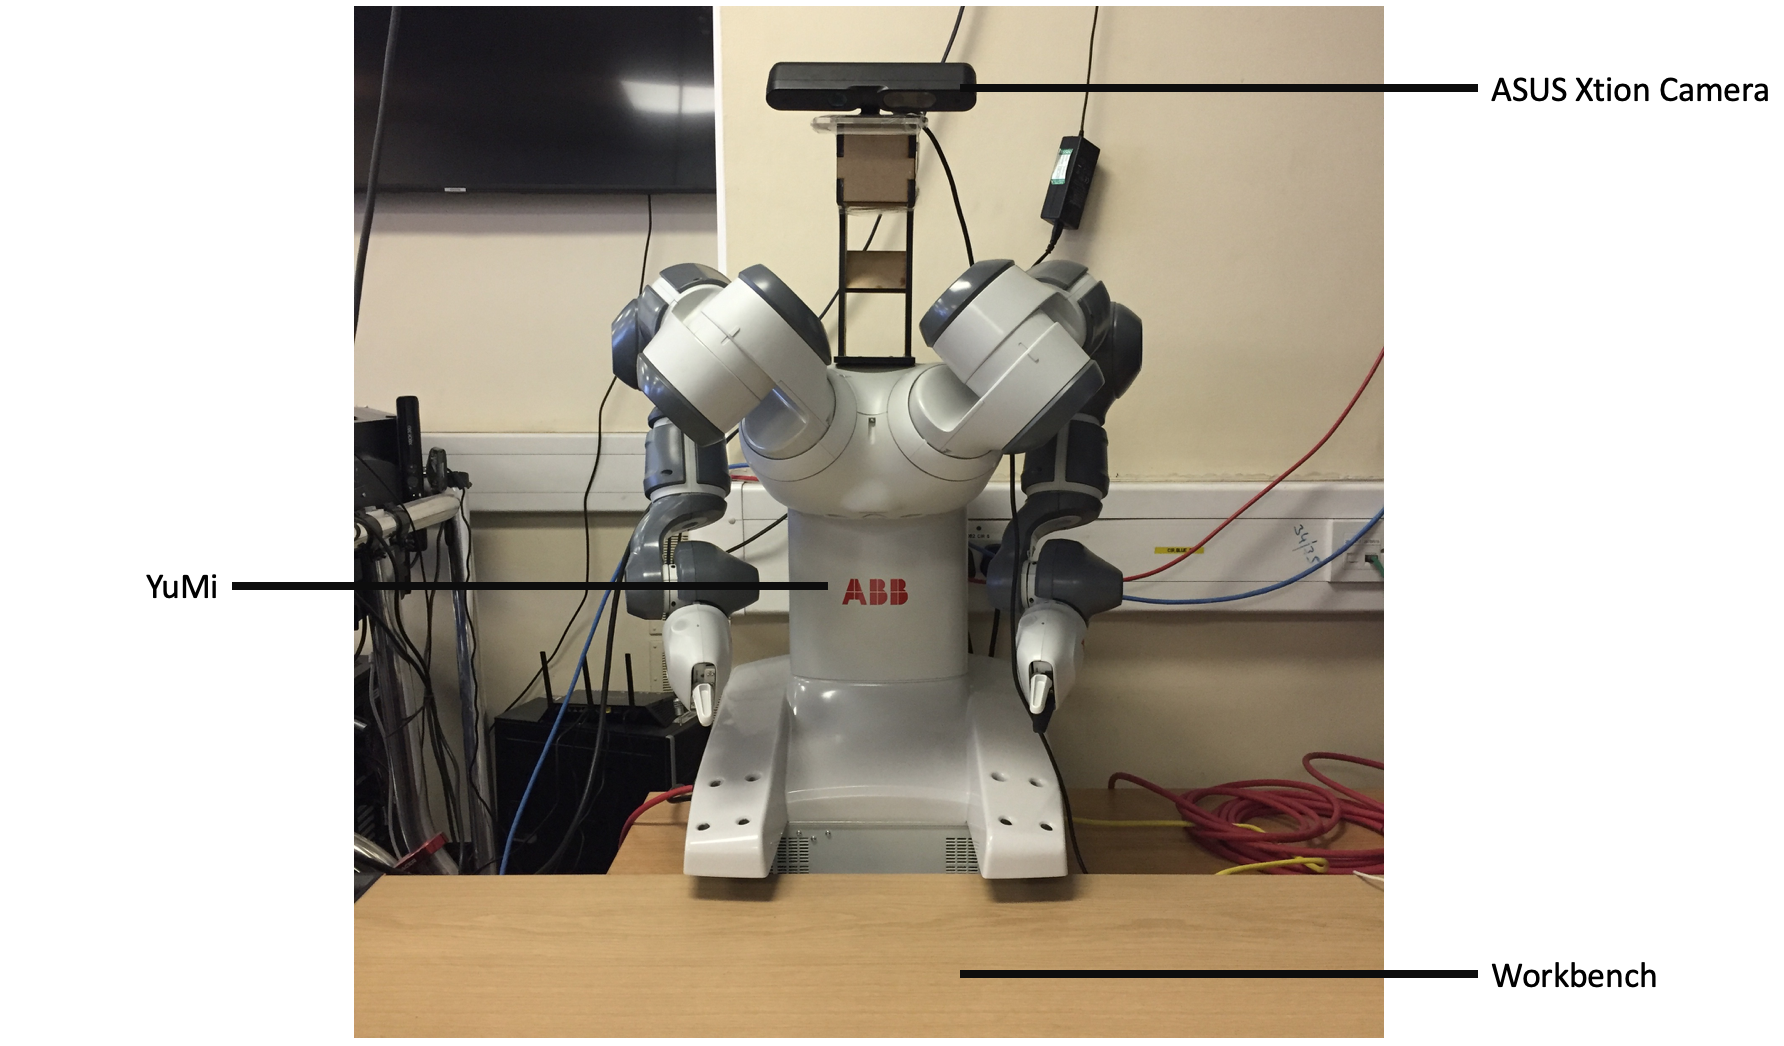
\includegraphics[width = \columnwidth]{Implementation/cv/yumicamera.png}
\caption{YuMi and ASUS Xtion camera position setup}
\label{5.1}
\end{figure}

Figure \ref{5.1} displays the relative position between YuMi and the two cameras. The cameras' location and orientation transform from YuMi frame $yumi\_base\_link$ are illustrated in Table \ref{cameraframeset} and written in the YuMi launch file (see !!!!!!!). These data are measured manually, which allow ROS $TF$ to perform frame transformation between any camera detected objects and YuMi in this project. 
\begin{table}[H]
\centering
\resizebox{\columnwidth}{!}{
\begin{tabular}{||c||c|c||}
\hline
Camera & Camera frame & Transform from $yumi\_base\_link$ \\ \hline\hline
ASUS Xtion & /camera\_link & {[}0.2013, 0.0641, 0.6934, -0.0238, 0.4836, -0.0141, 0.875{]} \\ \hline
ZED Mini & /zed\_left\_camera\_frame & {[}0.2263, 0.0541, 0.7134, -0.0238, 0.4836, -0.0141, 0.875{]} \\ \hline
\end{tabular}
}
\caption{Transform settings between YuMi and cameras}
\label{cameraframeset}
\end{table}

\section{Shoe Detection} \label{shoedetection}
As mentioned in Background Chapter, YOLO9000 will be used for shoe detection. \citep{bjelonicYolo2018} developed the YOLO ROS interface called $darknet\_ros$, which supports using YOLO on both CPU and GPU. This package depends on OpenCV, boost (C++ library) and CUDA (if use Nvidia GPU for faster processing). Detailed installation and setup instructions can be found in User Guide Chapter. 

\begin{figure}[H]
\centering

\includegraphics[width = 0.5\columnwidth]{images/ph.png}
\caption{Important files in Yolo package}
\label{yolofolder}
\end{figure}

By adding different version of $.weights$ and $.cfg$ files, creating corresponding configuration file ($yolo.yaml$), then pointing to the new $yolo.yaml$ file in the $darknet\_ros$ launch file, different version of YOLO can be used. Here, YOLO9000 is the choice.

\begin{figure}[H]
\centering
\subfigure[RGB raw image]{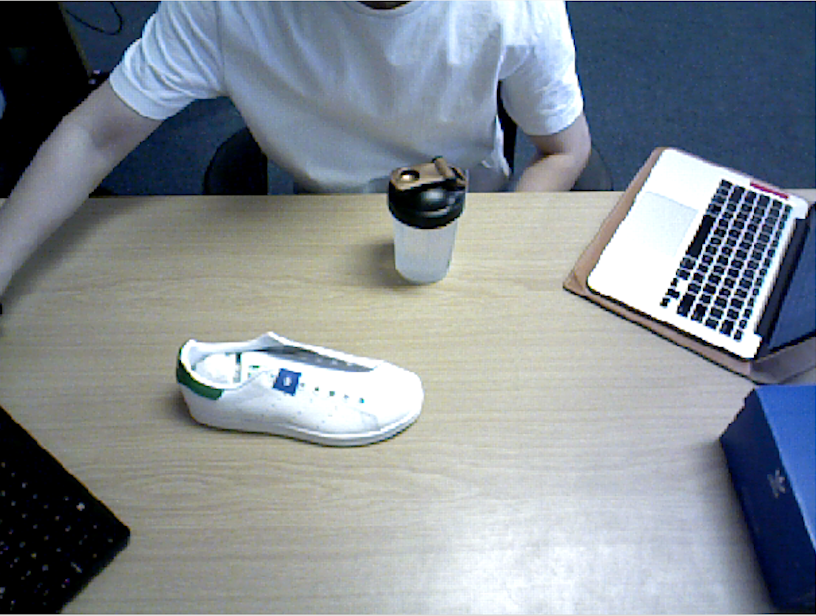
\includegraphics[width = 0.45\columnwidth]{Implementation/cv/raw.png}}
\subfigure[YOLO detection image including bounding boxes]{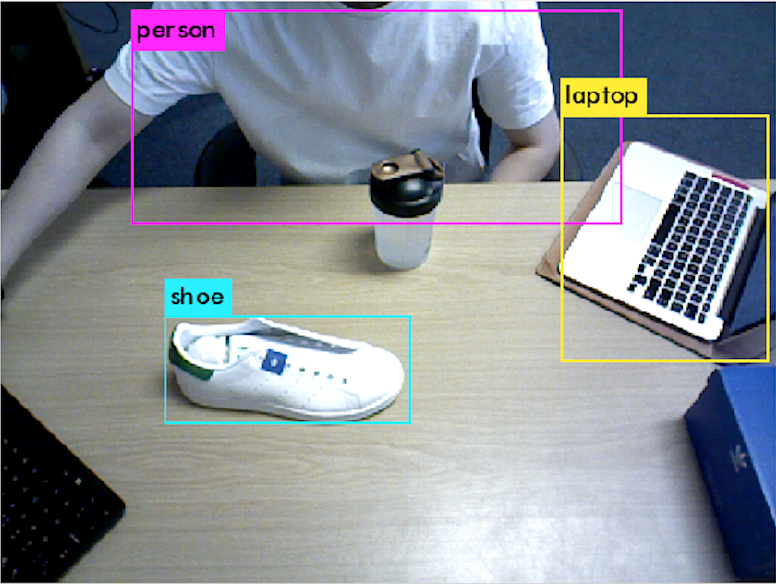
\includegraphics[width = 0.45\columnwidth]{Implementation/cv/yolo.png}}
\caption{Camera image before and after YOLO detection system}
\label{5.2}
\end{figure}

In the $yolo.yaml$ file, the threshold value is set to 0.3, which means the results will be reported only if the prediction probability of detection classes exceeds this value. The file named $ros.yaml$ defines the names and some parameters of the publishers, subscribers and actions of $darknet\_ros$. Here, the input is set as camera topic $/camera/rgb/image\_raw$, which contains raw RGB images taken by ASUS Xtion. It publishes several topics but only $/darknet\_ros/bounding\_boxes$ will be used in the following algorithms. The messages in this topic include the prediction class names of objects, their prediction probabilities and 2D bounding box coordinates ($xmin$, $xmax$, $ymin$, and $ymax$). If the category is predicted as 'shoe', the corresponding box coordinates will be recorded. By speeding up with GPU, $darknet\_ros$ can update the detection results approximately every 0.05 seconds.

\begin{figure}[H]
\centering
\subfigure[]{
\includegraphics[width = 0.15\columnwidth]{images/ph.png}}
\subfigure[]{
\includegraphics[width = 0.15\columnwidth]{images/ph.png}}
\subfigure[]{
\includegraphics[width = 0.15\columnwidth]{images/ph.png} \label{ver1}}
\subfigure[]{
\includegraphics[width = 0.15\columnwidth]{images/ph.png} \label{ver2}}
\subfigure[]{
\includegraphics[width = 0.15\columnwidth]{images/ph.png}}
\subfigure[]{
\includegraphics[width = 0.15\columnwidth]{images/ph.png}}
\caption{Examples of possible shoe orientations}
\end{figure}

In addition, the shoe can be placed in different directions, making the real manipulation difficult in some cases, especially when it is vertically placed (Figure \ref{ver1} and \ref{ver2}). Therefore, under this circumstance, its orientation need to be adjusted. To achieve that, the 2D coordinates 'around' the shoe bounding box will be documented (code!!!!!!!!!!!!!!!!!!!!!!) and detailed adjustment implementation can be found in Section \ref{adj}. After adjustment, the direction of the shoe and the interested shoe hole is considered to be toward the side of the camera.

\section{Required Locations for Shoe Pose Adjustment:}

\section{Shoe Hole Tracking}
Since the shoe is marked, shoe hole detection can be achieved with color detection. Due to the fact that color tracking is very sensitive to light condition, perform this technique using entire image cannot provide accurate results. Therefore, the image will firstly be cropped using $xmin$, $xmax$, $ymin$, and $ymax$ value computed in previous section. Color detection only applies to the cropped region of interest.

\begin{figure}[H]
\centering
\subfigure{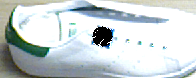
\includegraphics[width = 0.24\columnwidth]{Implementation/cv/bi1.png}}
\subfigure{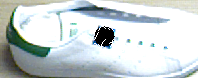
\includegraphics[width = 0.24\columnwidth]{Implementation/cv/g1.png}}
\subfigure{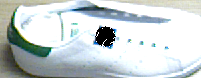
\includegraphics[width = 0.24\columnwidth]{Implementation/cv/m1.png}}
\subfigure{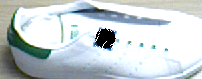
\includegraphics[width = 0.24\columnwidth]{Implementation/cv/b1.png}}

\subfigure{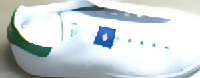
\includegraphics[width = 0.24\columnwidth]{Implementation/cv/bi2.png}}
\subfigure{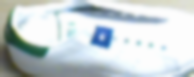
\includegraphics[width = 0.24\columnwidth]{Implementation/cv/g2.png}}
\subfigure{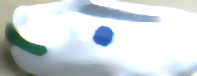
\includegraphics[width = 0.24\columnwidth]{Implementation/cv/m2.png}}
\subfigure{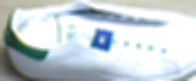
\includegraphics[width = 0.24\columnwidth]{Implementation/cv/b2.png}}

\subfigure{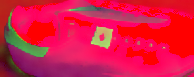
\includegraphics[width = 0.24\columnwidth]{Implementation/cv/bi3.png}}
\subfigure{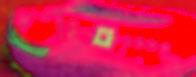
\includegraphics[width = 0.24\columnwidth]{Implementation/cv/g3.png}}
\subfigure{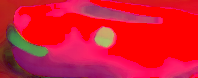
\includegraphics[width = 0.24\columnwidth]{Implementation/cv/m3.png}}
\subfigure{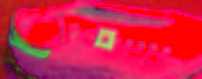
\includegraphics[width = 0.24\columnwidth]{Implementation/cv/b3.png}}

\subfigure{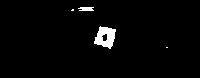
\includegraphics[width = 0.24\columnwidth]{Implementation/cv/bi4.png}}
\subfigure{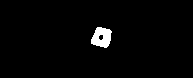
\includegraphics[width = 0.24\columnwidth]{Implementation/cv/g4.png}}
\subfigure{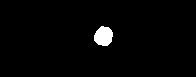
\includegraphics[width = 0.24\columnwidth]{Implementation/cv/m4.png}}
\subfigure{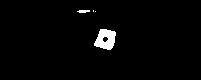
\includegraphics[width = 0.24\columnwidth]{Implementation/cv/b4.png}}

\subfigure{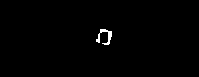
\includegraphics[width = 0.24\columnwidth]{Implementation/cv/bi5.png}}
\subfigure{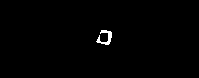
\includegraphics[width = 0.24\columnwidth]{Implementation/cv/g5.png}}
\subfigure{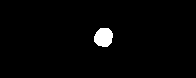
\includegraphics[width = 0.24\columnwidth]{Implementation/cv/m5.png}}
\subfigure{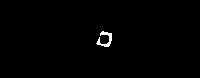
\includegraphics[width = 0.24\columnwidth]{Implementation/cv/b5.png}}

\subfigure[Bilateral filter]{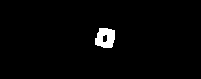
\includegraphics[width = 0.24\columnwidth]{Implementation/cv/bi6.png}}
\subfigure[Gaussian filter]{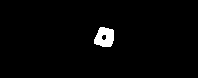
\includegraphics[width = 0.24\columnwidth]{Implementation/cv/g6.png}}
\subfigure[Median filter]{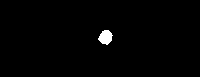
\includegraphics[width = 0.24\columnwidth]{Implementation/cv/m6.png}}
\subfigure[Normalized Box filter]{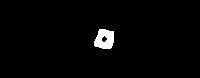
\includegraphics[width = 0.24\columnwidth]{Implementation/cv/b6.png}}
\caption{Image processing of extracted shoe region. Each column uses one specific type of blurred filter. For each column, from top to bottom, each image is, in turn, the original image labeled with detected contour area, smoothed image after applying the linear filter, image of HSV color space of the smoothed image, mask for color 'blue', mask after $erode$ function, and the final mask after $dilate$ function}
\label{filter}
\end{figure}

The image of shoe always contains a certain level of high frequency noise. Various blurring and smoothing techniques have been tried to tackle this issue (detail and reference !!!!!!!!!!!!) and their results are shown in Figure \ref{filter} second line. The blurred image is then converted to HSV color space. After that, a mask for color 'blue' is constructed using its predefined lower and color boundaries. The $erode$ and $dilate$ functions are then performed to remove any small blobs remain in the mask. It can be discovered that basically all the four filter can provide a reasonable mask of shoe hole area.

The contour(s) of blue area(s) are then calculated. If at least one contour is discovered, the largest one in the mask will be used and its centroid is computed accordingly. Noticed that this centroid coordinate is for the cropped image. Therefore, $xmin$ and $ymin$ must be added back to give the coordinate of the original $640 \times 480$ image. Finally, if the contour area lies between a predefined range, the calculated centroid will be regarded as the centroid of the shoe hole and used for further computation.

\section{3D Location of Shoe Hole} \label{3dlocationestimation}
Once the real-time 2D position of shoe hole is calculated, its real-world 3D location can be obtained by looking at $/camera/depth\_registered/points$ topic. This topic contains depth registered point clouds as shown in Figure \ref{ptcloud}. depth align!!!!!!!!!!!!!!!!

\begin{figure}[H]
\centering
\subfigure[RGB raw image]{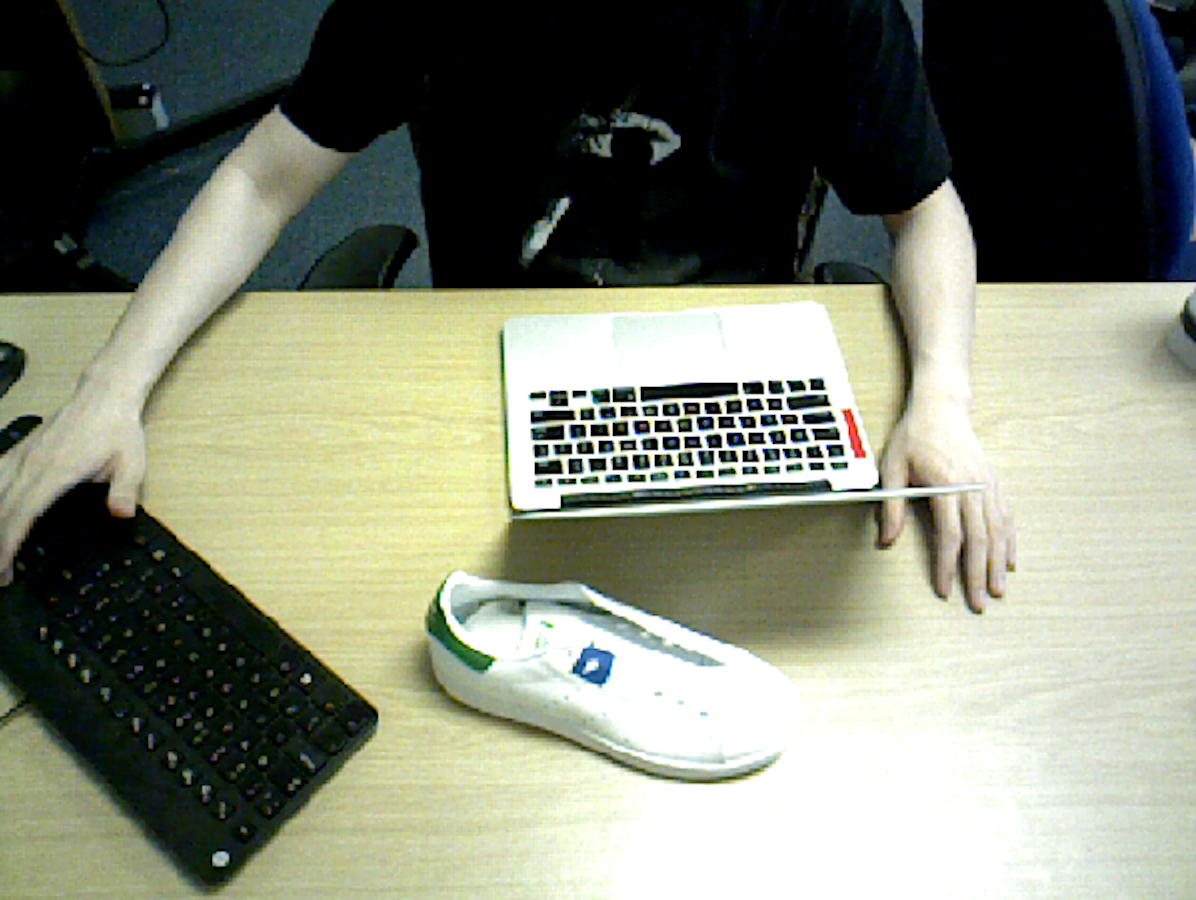
\includegraphics[width = 0.45\columnwidth, height=50mm]{Implementation/cv/rgbpt.png}}
\subfigure[Depth registered point clouds]{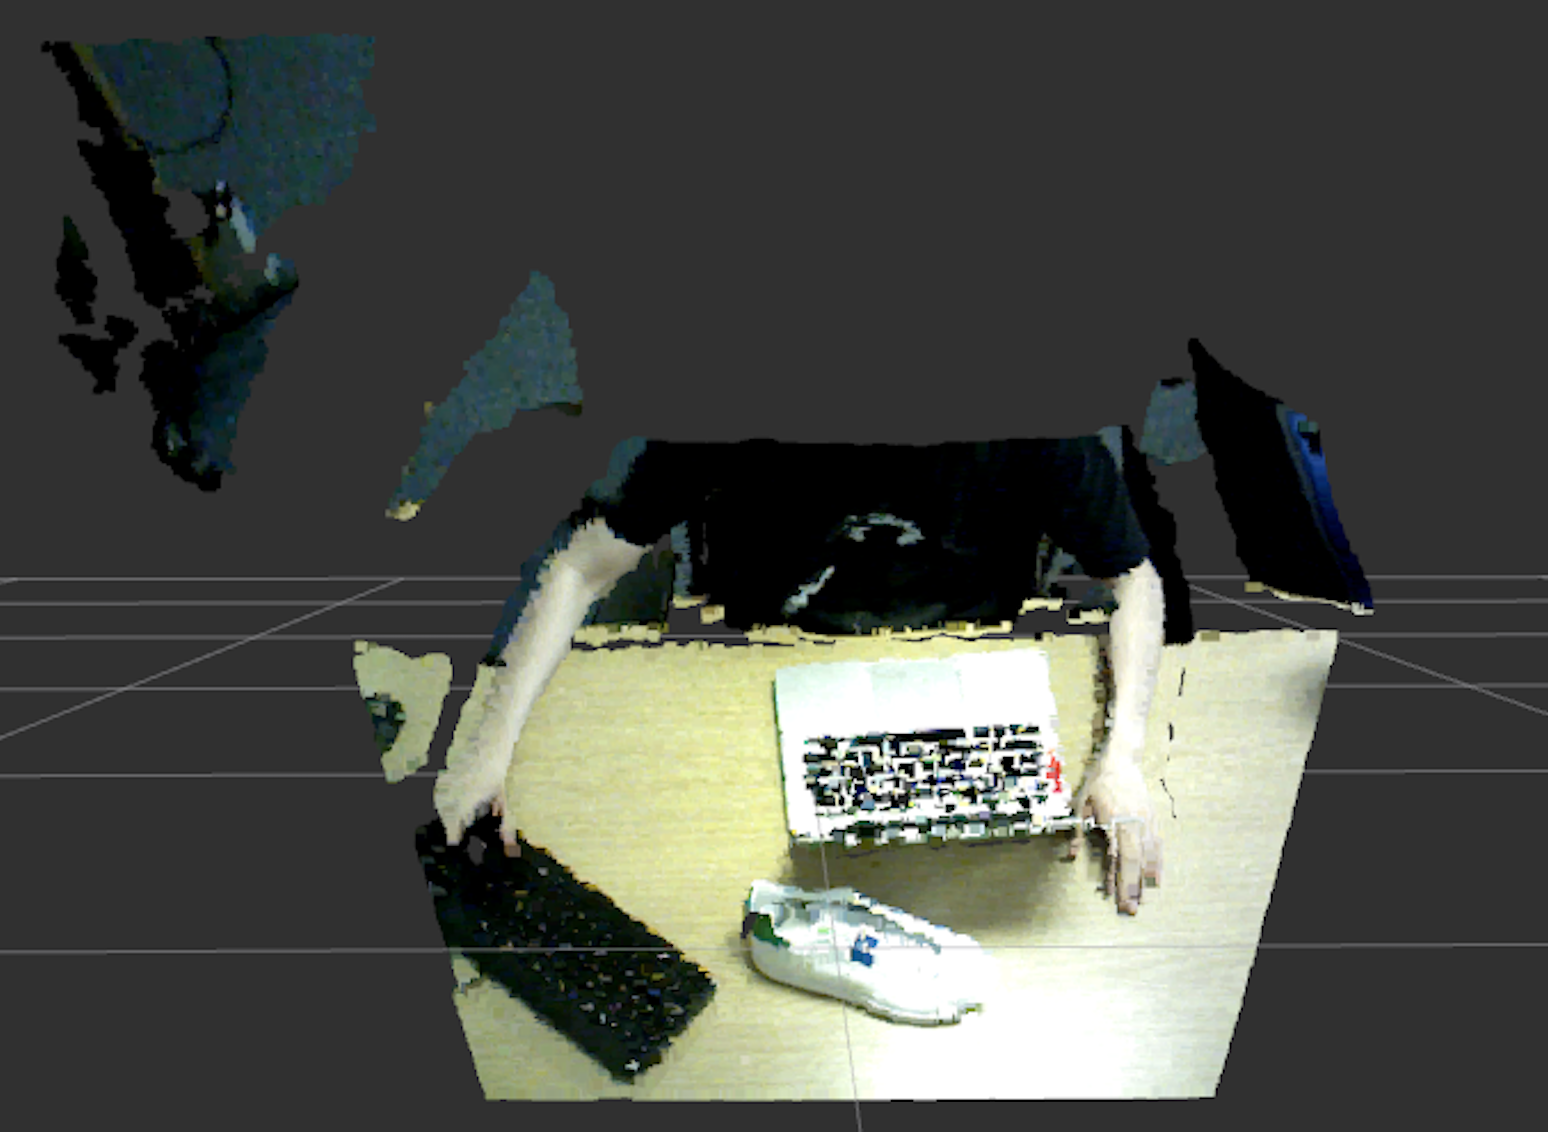
\includegraphics[width = 0.45\columnwidth, height=50mm]{Implementation/cv/ptcloud.png} \label{ptcloud}}
\caption{Messages of different camera topics}
\end{figure}

Each point cloud contains the real-world $xyz$ readings relative to the camera and RGB information. Since the image resolution of camera is $640 \times 480$, there are total $307200$ points for each image. Sometimes, the $xyz$ readings of some points might be $nan$, which are not reliable and need to be ignored. Using the 2D position ($self.cx, self.cy$) calculated in the previous section, $pc2.read\_points$ function helps the find corresponding point cloud and return the reading.

\begin{minted}[frame=single, framesep=1.5mm, baselinestretch=1, fontsize=\footnotesize, linenos, breaklines]{python}
data_out = pc2.read_points(data, field_names = ('x', 'y', 'z'), skip_nans = True, uvs = [(self.cx, self.cy)])
int_data = list(data_out)
if len(int_data) > 0:
    point_x, point_y, point_z = int_data[0]
    shoe_hole = [point_z, -point_x, -point_y]
    self._tfpub.sendTransform((shoe_hole), tf.transformations.quaternion_from_euler(0, 0, 0), rospy.Time.now(), "shoe_hole", 'camera_link')
\end{minted}

Notice that the reading is based on camera frame called $camera\_link$ and camera axes. In order to move YuMi's arm around this location in later stages accordingly, the reading needs to be related to YuMi frame $yumi\_body$ and using YuMi axes format. The relationship between their axes is illustrated in line 5 of the code, $shoe\_hole$ is the location in YuMi axes. As mentioned in Analysis and Design Chapter, $TF$ keeps the relationship between frames, which is used for the frame conversion. The location $shoe\_hole$ is firstly published using $sendTransdorm$ function, as a transform from frame $camera\_link$. Then function $lookupTransform$ can be used to obtained the location based on frame $yumi\_body$, which will be further discussed in next Chapter. Figure \ref{3dpos} shows these frames visualized in Rviz.

\begin{figure}[H]
\centering
\subfigure[Real-world shoe placement]{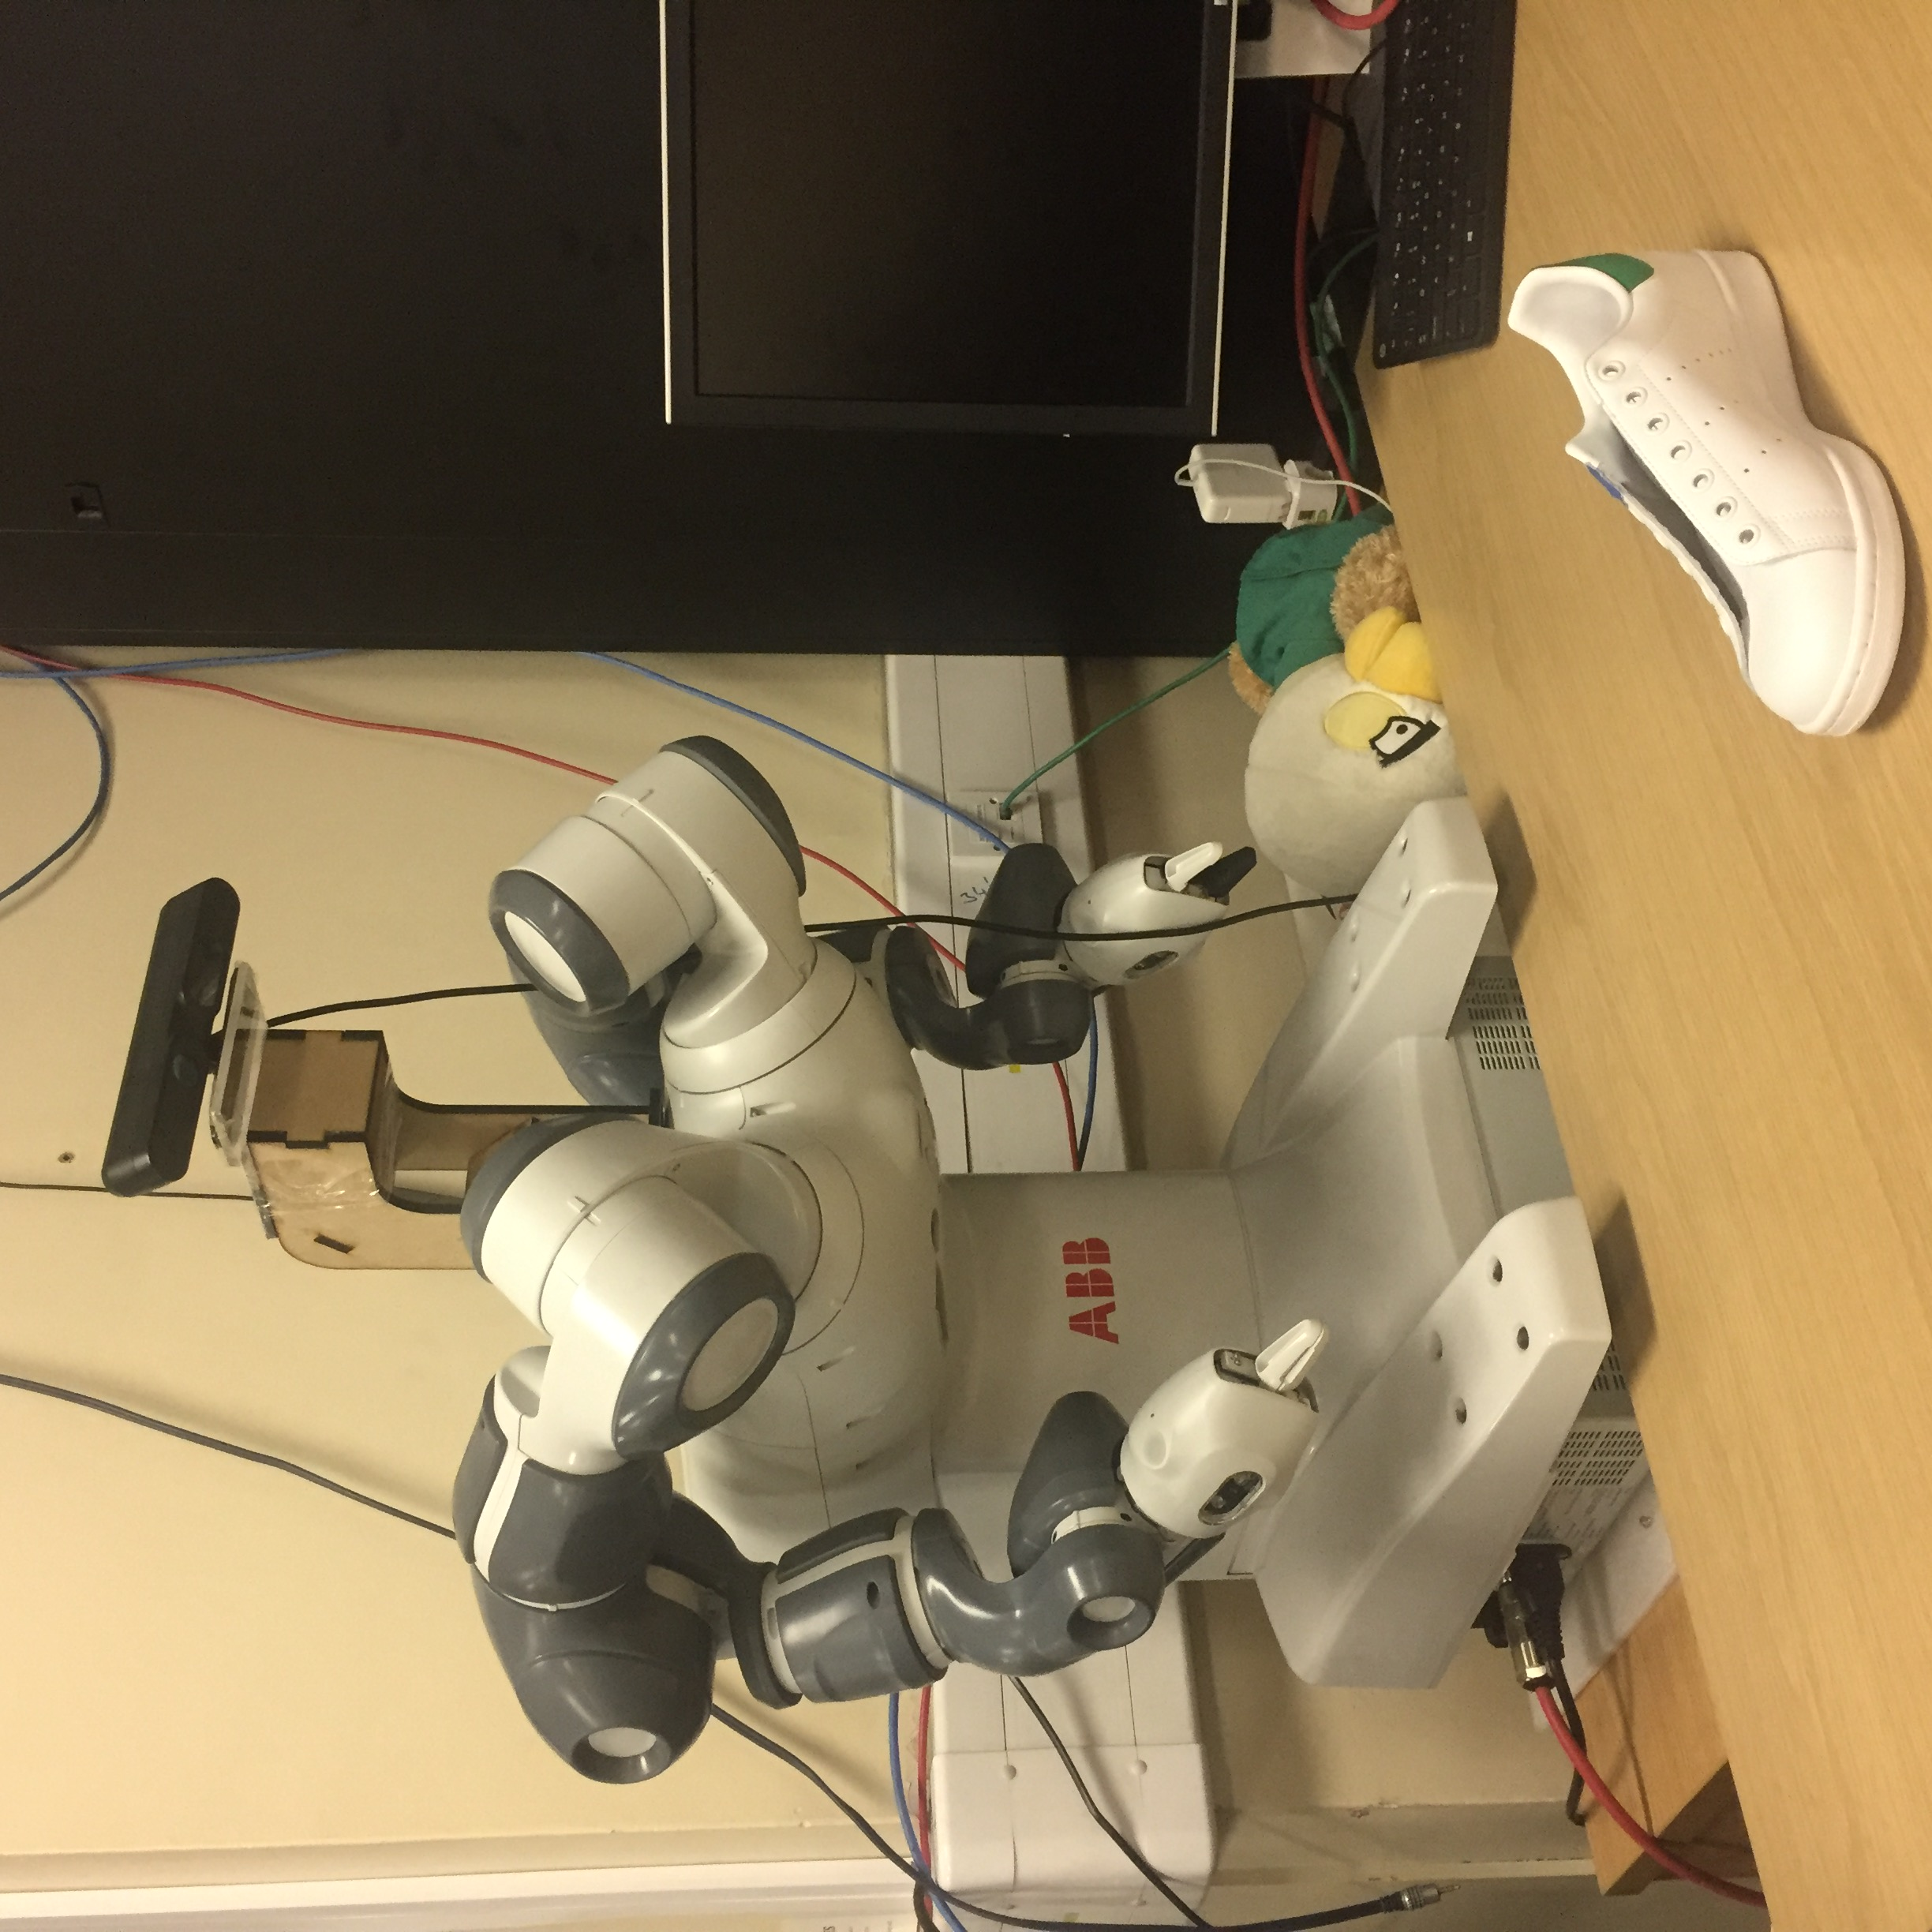
\includegraphics[angle=270, origin=c, width = 0.45\columnwidth]{Implementation/cv/3dposw.JPG}}
\subfigure[The frame relationships in Rviz]{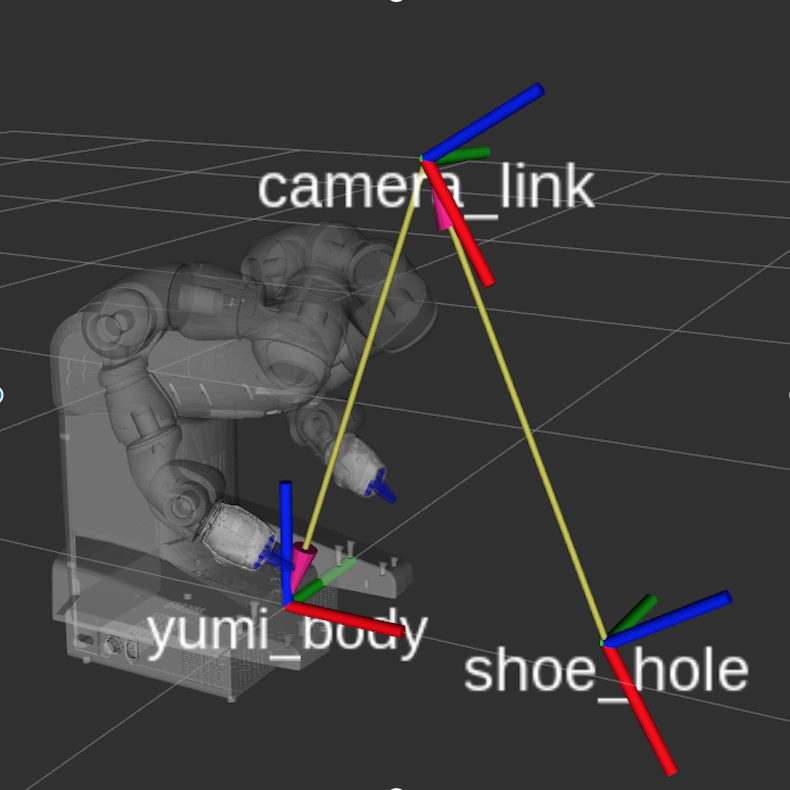
\includegraphics[width = 0.45\columnwidth]{Implementation/cv/3dpos.png} \label{3dpos}}
\caption{Example of shoe hole 3D location estimation}
\end{figure}

\section{3D Orientation of Shoe Hole}
Due to the fact that the surrounding area of the shoe hole can be regarded as a plane, as shown in Figure \ref{plane}, its 3D orientation is the same as that of the plane. In addition, the orientation of a plane can be obtained from its plane equation. For a plane $Ax + By + Cz = D$, its normal vector is $n = Ai + Bj + Ck$.

\begin{figure}[H]
\centering
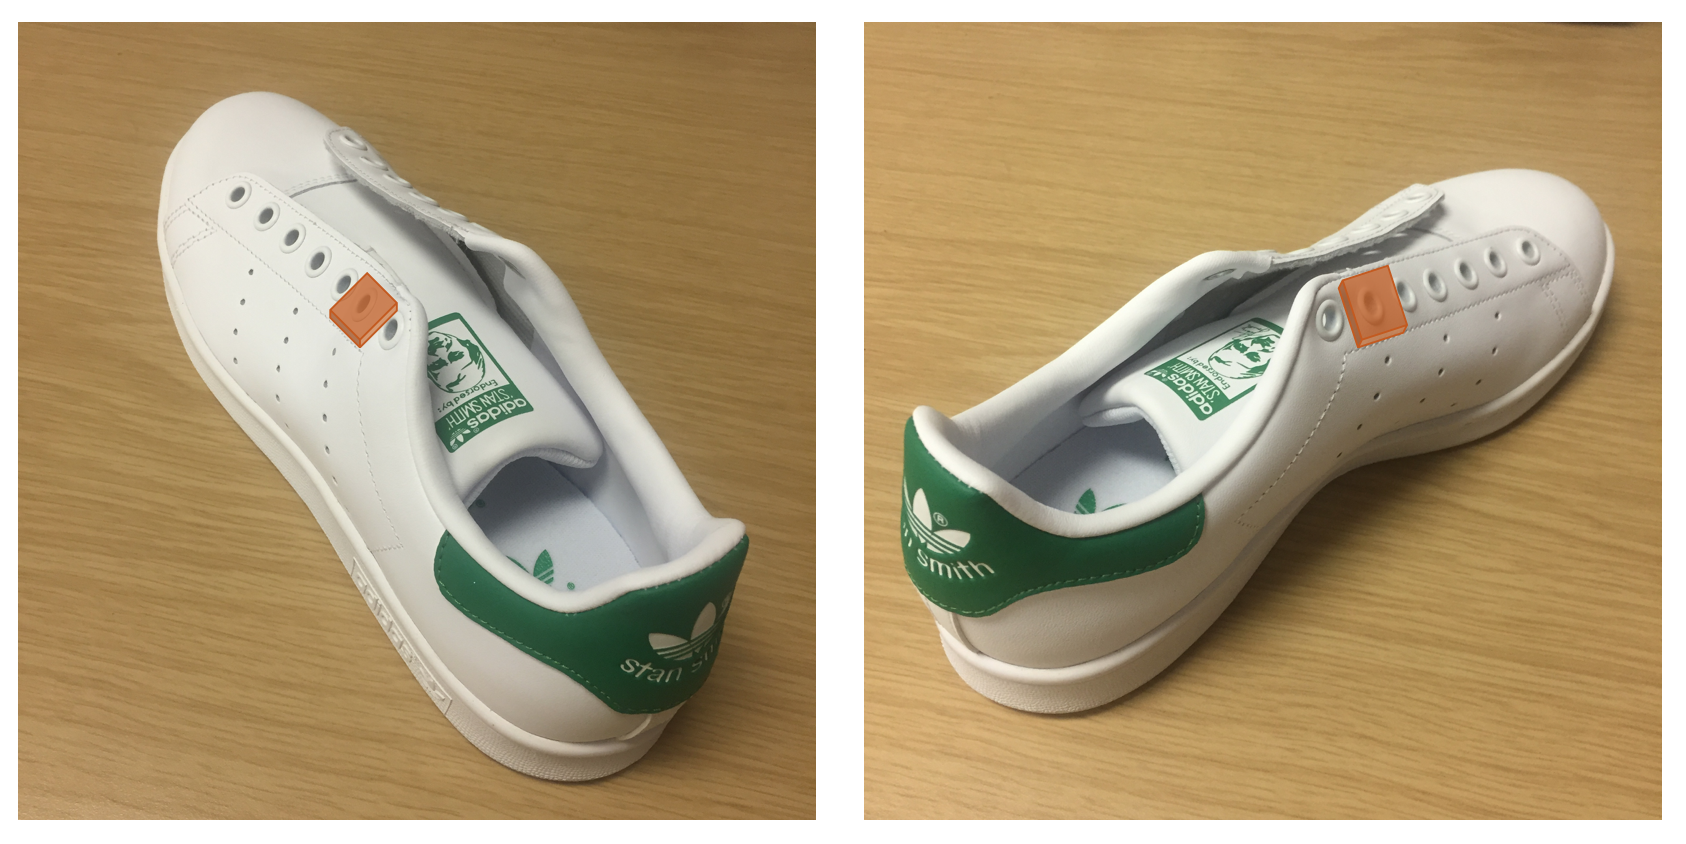
\includegraphics[width = 0.9\columnwidth]{Implementation/cv/plane.png}
\caption{The surrounding area of the shoe hole. The orientation of the orange plane is approximately same as that of the shoe hole within it.}
\label{plane}
\end{figure}

As mentioned in Background Chapter, by extracting all the surrounding point clouds of the shoe hole, RANSAC can then be applied to estimate the plane parameters A, B, C, and D, while ignoring the outliers. Here, a square with a side length of 10 pixels centered on the shoe hole is regarded as the reasonable surrounding area. Taking these 100 points as input, following settings are used for RANSAC.

\begin{table}[H]
\centering
\begin{tabular}{||c|c|c||}
\hline
Number of hypothetical inliers & Distance threshold & Max iterations \\ \hline\hline
20 & 0.01 & 200 \\ \hline
\end{tabular}
\caption{RANSAC parameters setting}
\label{ransacsetting}
\end{table}

Again, the output parameters are referenced to $camera\_link$, whose direction points into the shoe. However, the expected normal vector should be facing away from the shoe so that the YuMi gripper can insert the lace into the hole in this direction. This conversion is achieved by simply multiplying every plane coefficient by $-1$. In addition, I defined a pre-insertion point called $norm\_shoe\_hole$ along the normal vector direction, so that YuMi moves its gripper to this position, then aligns the gripper with the normal vector, and finally moves to $shoe\_hole$. Location $norm\_shoe\_hole$ can be represented as $(-0.1*A, -0.1*B, -0.1*C)$ referenced to $shoe\_hole$.

Another issue of this approach is that $norm\_shoe\_hole$ has great volatility. The readings fluctuate every time, which are extremely unstable. To tackle this, I firstly introduced a constraint. Since the orientation of the shoe hole is supposed to toward camera side, the x coordinate of $norm\_shoe\_hole$ must be smaller than that of the $shoe\_hole$. Therefore, the algorithm will ignore any calculated vector with unreasonable x coordinates. To further improve the stability and accuracy of the results, every 50 vector coefficients will be recorded and further data processing will be performed. The following two techniques have been experimented. 

\begin{itemize}
    \item \textbf{K-means Clustering:} K-means can partition these 50 $norm\_shoe\_hole$ into k clusters where each point belongs to the cluster with the nearest mean. The cluster with the most number of points will be treated as the correct one and the cluster mean is the final $norm\_shoe\_hole$s. However, for this approach, the number of cluster need to be defined at first. Different settings give very different results even under same environments. Once the selected cluster is wrong, the resulting point can be ridiculous sometimes, which is unreliable.
    
    \item \textbf{Average:} Considering the majority of calculated points are reliable, averaging these 50 $norm\_shoe\_hole$ should give a reasonable answer. This method has been experimented and proven to be effective.
\end{itemize}

The final $norm\_shoe\_hole$ are then be published to $TF$ topic as a transform from frame $shoe\_hole$. Figure \ref{3dori} illustrates all the frames used up to this stage.

\begin{figure}[H]
\centering
\subfigure[Real-world shoe placement]{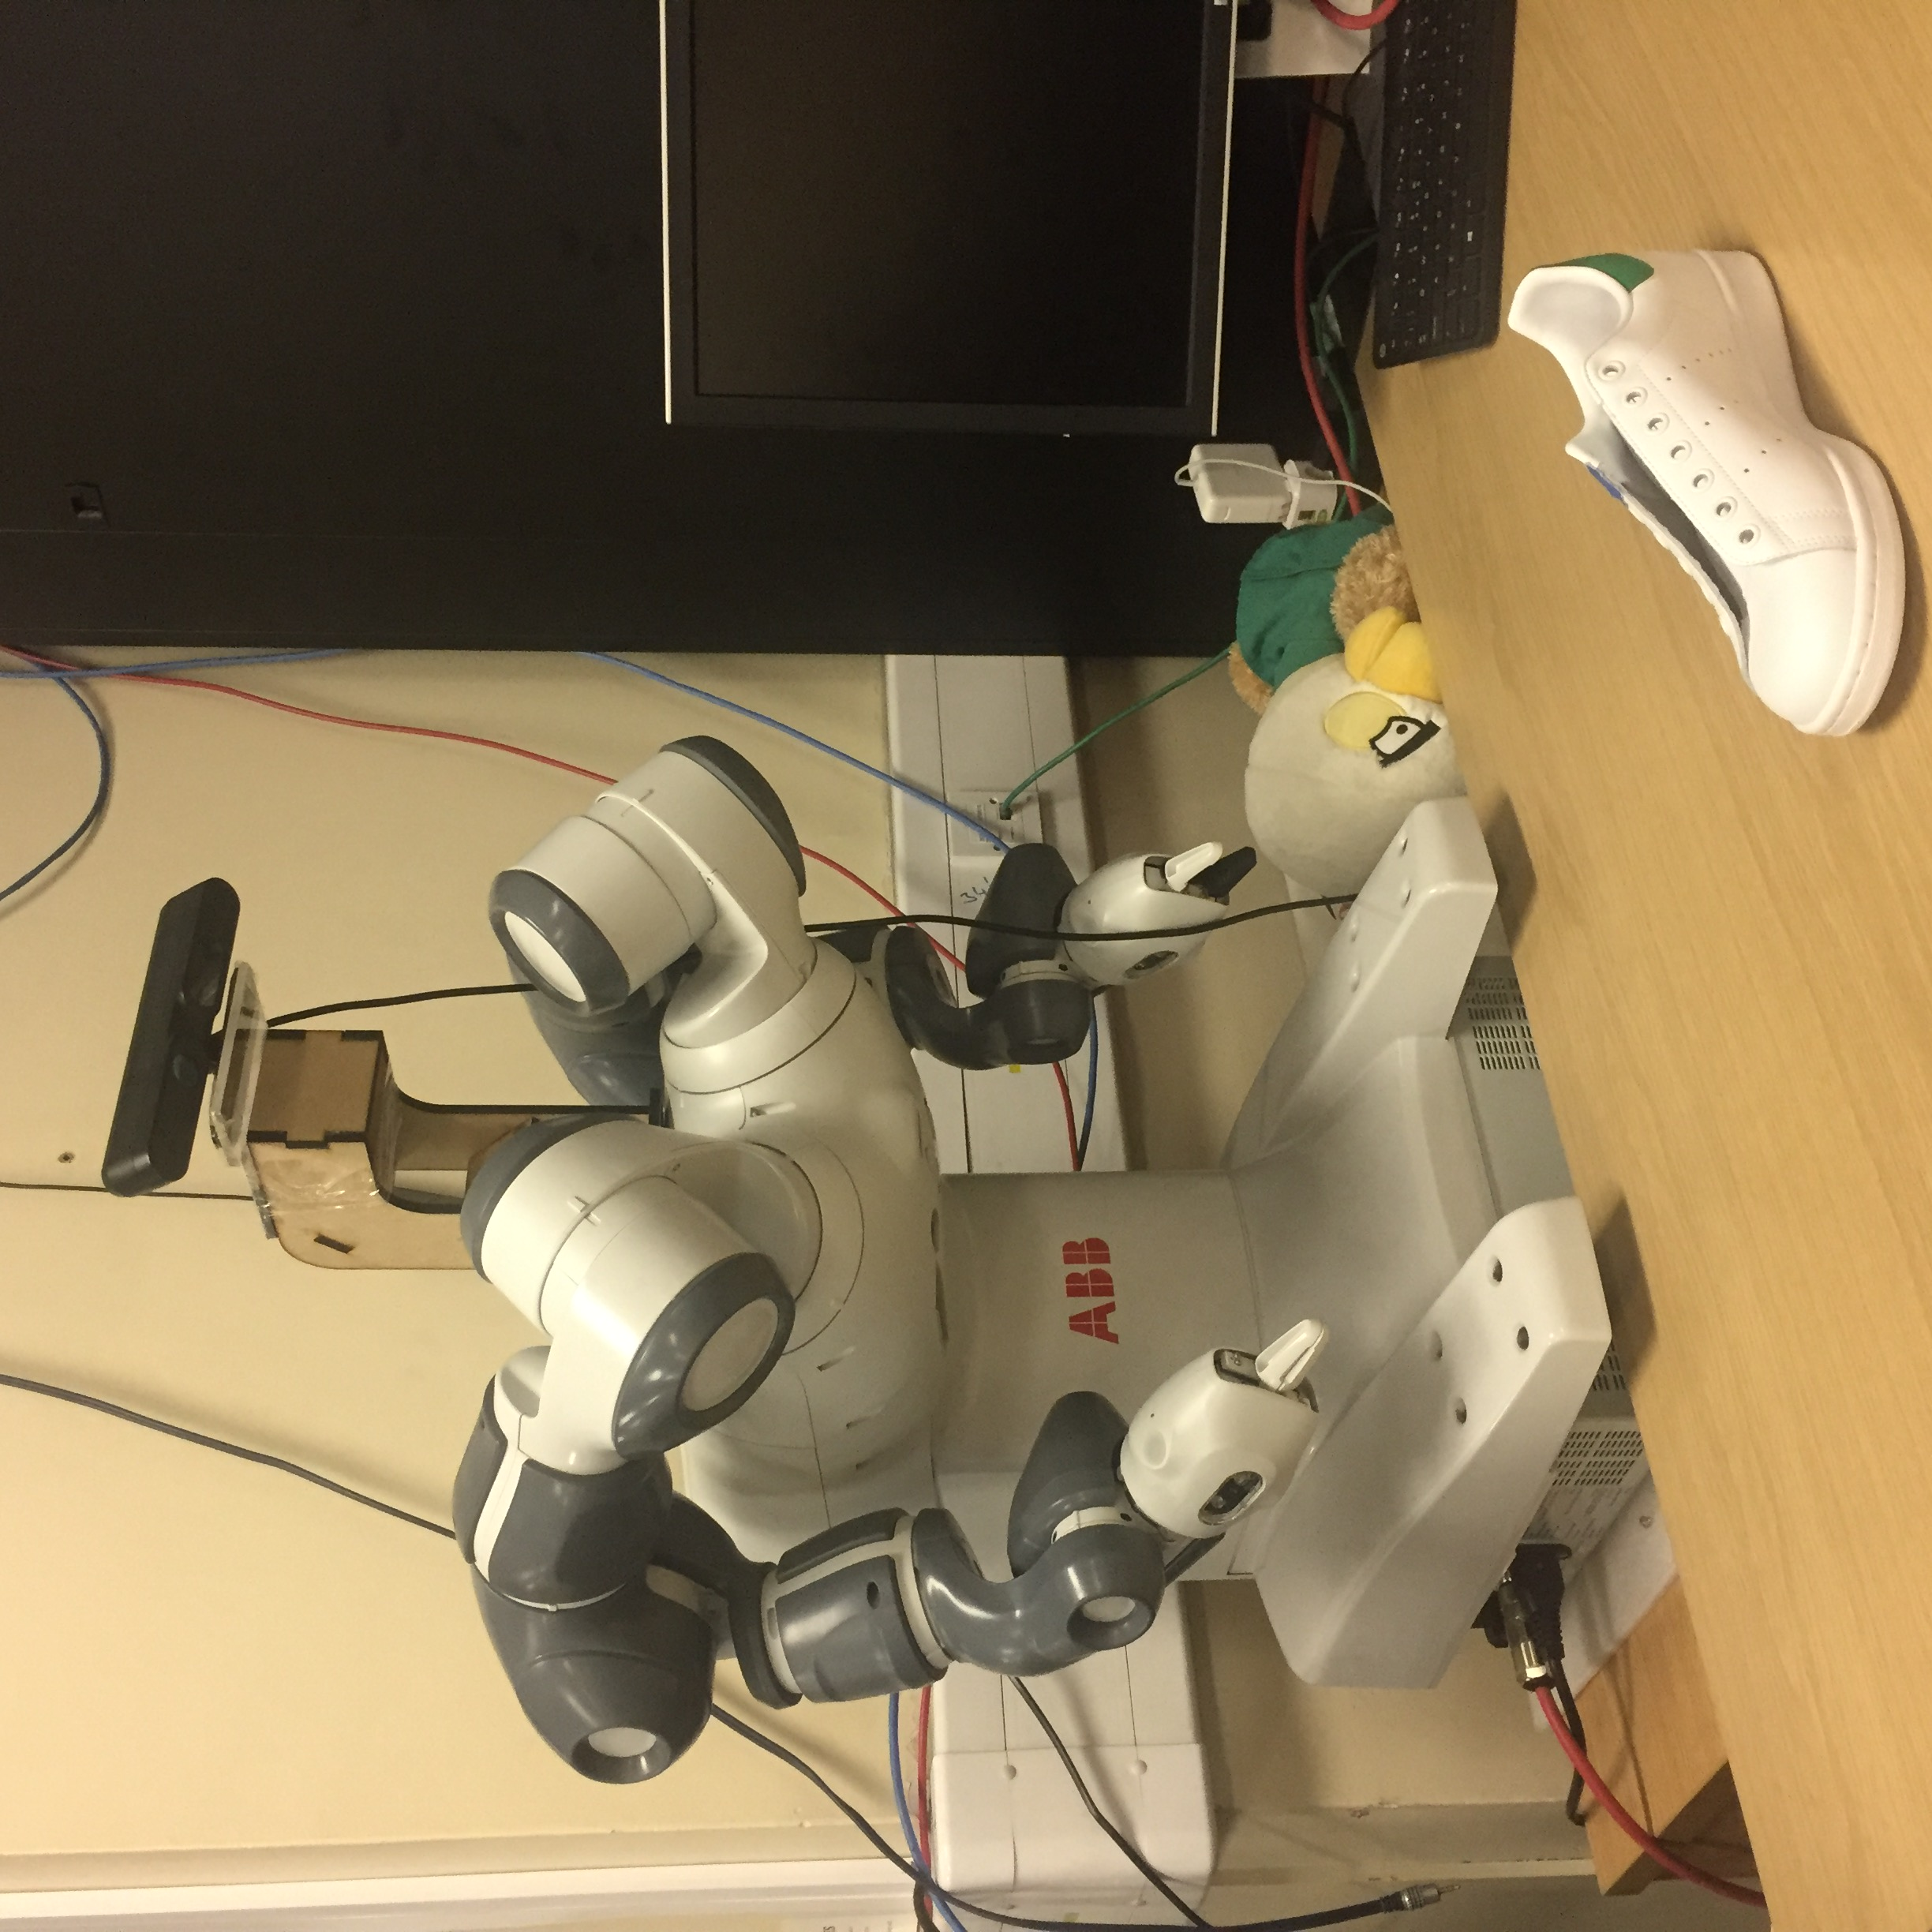
\includegraphics[angle=270, origin=c, width = 0.45\columnwidth]{Implementation/cv/3dposw.JPG}}
\subfigure[The frame relationships in Rviz]{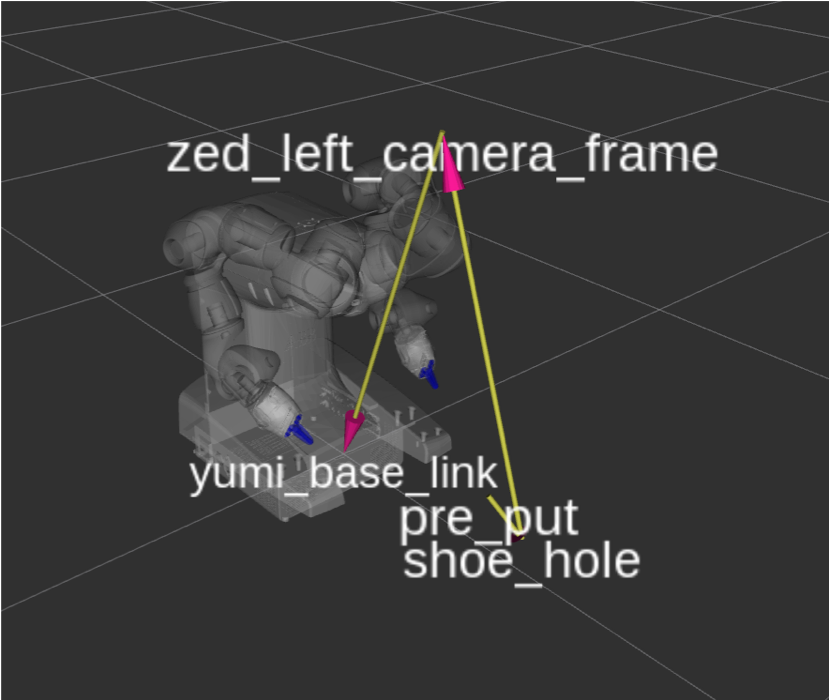
\includegraphics[width = 0.45\columnwidth]{Implementation/cv/3dori.png}\label{3dori}}
\caption{Example of shoe hole 3D orientation estimation}
\end{figure}


\section{3D Orientation of Shoelace}